
\textbf{LLVM中的Pass}是对LLVM IR执行某些操作所必需的基本单元。这类似于工厂的单个生产步骤,需要加工的产品是LLVM IR,工厂的工人就是Pass。就像一个普通的工厂通常有多个制造步骤一样,LLVM也包含多个按顺序执行的Pass,称为\textbf{Pass流水}。图9.1展示了Pass管道的一个例子:

\hspace*{\fill} \\ %插入空行
\begin{center}
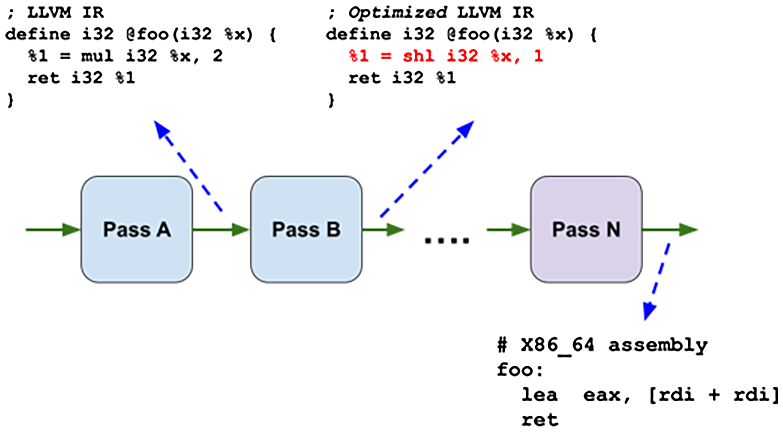
\includegraphics[width=0.9\textwidth]{content/3/chapter9/images/1.png}\\
图9.1 - LLVM Pass流水的例子及其中间结果
\end{center}

上图中,多个通道沿一条直线排列。一个又一个Pass处理\texttt{foo}函数的LLVM IR,例如:Pass B对\texttt{foo}执行代码优化,用左移(\texttt{shl})1替换算术乘法(\texttt{mul})2,在大多数硬件体系结构中,认为位移比乘法更快。此外,该图还说明了\textbf{代码生成}步骤建模为Pass。LLVM中的代码生成将LLVM IR(与目标无关)转换成特定硬件架构的汇编代码(图9.1中的\textbf{x86\_6}4)。每个详细的过程,比如:寄存器分配、指令选择或指令调度,都封装在一个Pass中,并按照一定的顺序执行。

\begin{tcolorbox}[colback=blue!5!white,colframe=blue!75!black, fonttitle=\bfseries,title=代码生成Pass]	
\hspace*{0.7cm}用于代码生成的Pass具有与普通LLVM IR Pass不同的API。在代码生成阶段,LLVM IR实际上转换成另一种IR,称为\textbf{Machine IR (MIR)}。本章中,我们只讨论LLVM IR和它的Pass。
\end{tcolorbox}

这个Pass流水在概念上是由\texttt{PassManager的}的基础设施管理。PassManager拥有运行这些Pass的计划——例如:执行顺序。通常,交替使用术语\textit{Pass pipeline}和\textit{PassManager},因为它们有几乎相同的任务。在后面的小节中,我们将更详细地介绍流水本身,并讨论如何定制这些封装Pass的执行顺序。

现代编译器中的代码转换可能很复杂。因此,多个转换Pass可能需要相同的一组程序信息,这在LLVM中称为\textbf{分析},以完成它们的工作。此外,为了实现效率最大话,LLVM还缓存这些分析数据,以便在可能的情况下重用这些数据。但是,由于转换Pass可能会更改IR,一些缓存的分析数据(以前收集的)在运行该Pass之后就会过期。为了解决这些挑战,除了PassManager之外,LLVM还创建了\textbf{AnalysisManager}来管理与程序分析相关的一切。

如本章介绍中提到的,LLVM已经对其Pass和PassManager(以及AnalysisManager)基础设施进行了一系列的检查。新的基础设施运行得更快,产生的结果质量更好。然而,新Pass在许多地方与旧的不同,我们将简要解释这些差异。除此之外,本章的其余部分,将只讨论新Pass的基础架构。

在本节中,我们将展示如何为新PassManager开发一个简单的Pass。与往常一样,我们将从描述将要使用的示例项目开始。然后,展示创建Pass的步骤,该Pass可以使用\texttt{opt}从插件动态加载到Pass管道中(前面提到过)。

\subsubsubsection{9.2.1\hspace{0.2cm}项目概述}

本节中,使用的示例项目称为\textbf{StrictOpt}。它是一个Pass和Pass插件,为每个具有指针类型的函数形参添加\texttt{noalias}属性。实际上,它向C代码中的函数参数添加了一个\texttt{restrict}关键字。首先,让我们了解一下\texttt{restrict}关键字的作用。

\begin{tcolorbox}[colback=blue!5!white,colframe=blue!75!black, fonttitle=\bfseries,title=C和C++中的restrict关键字]	
\hspace*{0.7cm}C99中引入了\texttt{restrict}关键字。然而,它在C++中没有对应的关键字。尽管如此,主流编译器如Clang、GCC和MSVS在C++中都支持相同的功能。例如,在Clang和GCC中,可以在C++代码中使用\texttt{\_\_restrict\_\_}或\texttt{\_\_restrict},效果与C中的\texttt{restrict}相同。
\end{tcolorbox}

C语言中,\texttt{restrict}关键字可以与指针类型变量一起使用。在最常见的情况是,与指针类型的函数形参一起使用。示例如下:

\begin{lstlisting}[style=styleCXX]
int foo(int* restrict x, int* restrict y) {
	*x = *y + 1;
	return *y;
}
\end{lstlisting}

这个属性会告诉编译器,参数\texttt{x}永远不会指向与参数\texttt{y}相同的内存区域。换句话说,程序员可以使用这个关键字来说服编译器,他们永远不会像这样使用\texttt{foo}函数,如下所示:

\begin{lstlisting}[style=styleCXX]
…
// Programmers will NEVER write the following code
int main() {
	int V = 1;
	return foo(&V, &V);
}
\end{lstlisting}

这背后的基本原理是,如果编译器知道两个指针——本例中,两个指针参数——永远不会指向同一个内存区域,它就可以进行更积极的进行优化。更具体的理解是,如果比较\texttt{foo}函数的汇编代码与限制关键字和不限制关键字,后一个版本需要执行5条指令(在\textbf{x86\_64}上):

\begin{lstlisting}[style=stylePython]
foo:
	mov eax, dword ptr [rsi]
	add eax, 1
	mov dword ptr [rdi], eax
	mov eax, dword ptr [rsi]
	ret
\end{lstlisting}

添加\texttt{restrict}关键字的版本只有四条指令:

\begin{lstlisting}[style=stylePython]
foo:
	mov eax, dword ptr [rsi]
	lea ecx, [rax + 1]
	mov dword ptr [rdi], ecx
	ret
\end{lstlisting}

尽管这里的区别看起来很微妙,但在没有\texttt{restrict}的版本中,编译器需要插入额外的内存负载,以确保最后一个参数\texttt{*y}(在原始C代码中)总是读取最新的值。这些额外的成本可能会逐渐累积在更复杂的代码库中,并最终造成性能瓶颈。

现在,已经了解了\texttt{restrict}是如何工作的,以及对良好性能的重要性。在LLVM IR中,也有一个对应的指令来建模\texttt{restrict}关键字:\texttt{noalias}属性。如果原始源代码中给出了诸如\texttt{restrict}之类的提示,则该属性则会附加到指针函数参数上。例如,\texttt{foo}函数(带有\texttt{restrict}关键字),则翻译成如下LLVM IR:

\begin{lstlisting}[style=stylePython]
define i32 @foo(i32* noalias %0, i32* noalias %1) {
	%3 = load i32, i32* %1
	%4 = add i32 %3, 1
	store i32 %4, i32* %0
	ret i32 %3
}
\end{lstlisting}

此外,还可以在C代码中无\texttt{restrict}地生成\texttt{foo}函数的LLVM IR代码,如下所示:

\begin{lstlisting}[style=stylePython]
define i32 @foo(i32* %0, i32* %1) {
	%3 = load i32, i32* %1
	%4 = add i32 %3, 1
	store i32 %4, i32* %0
	%5 = load i32, i32* %1
	ret i32 %5
}
\end{lstlisting}

这里,将有一个额外的内存负载(如前面代码段突出显示的指令所示),这与前面的程序集示例的情况类似。也就是说,LLVM无法执行更积极的优化来移除内存负载,因为它不确定这些指针是否会重叠。

本节中,我们将编写一个Pass来为函数的每个指针参数添加\texttt{noalias}属性。Pass将作为插件构建,当它加载到\texttt{opt}中时,用户可以使用\texttt{-\,-passes}参数显式触发\texttt{StrictOpt},如下所示:

\begin{tcblisting}{commandshell={}}
$ opt --load-pass-plugin=StrictOpt.so \
      --passes="function(strict-opt)" \
      -S -o – test.ll
\end{tcblisting}

或者,如果优化级别大于或等于\texttt{-O3},可以在其他优化之前运行\texttt{StrictOpt}。示例如下:

\begin{tcblisting}{commandshell={}}
$ opt -O3 --enable-new-pm \
      --load-pass-plugin=StrictOpt.so \
      -S -o – test.ll
\end{tcblisting}

我们将展示如何在这两种模式之间进行切换。

\begin{tcolorbox}[colback=blue!5!white,colframe=blue!75!black, fonttitle=\bfseries,title=只是Pass的演示示例]	
\hspace*{0.7cm}注意,\texttt{StrictOpt}仅仅是Pass的演示示例,并且在每个指针函数参数中添加\texttt{noalias}绝对不是在实际用例中应该做的事情。因为这样做可能会破坏程序的正确性。
\end{tcolorbox}

下一节中,我们将展示如何创建此Pass的详细步骤。

\subsubsubsection{9.2.2\hspace{0.2cm}编写StrictOpt Pass}

介绍如何将\texttt{StrictOpt}动态注册到Pass管道之前,下面将说明开发核心Pass逻辑的整个过程:

\begin{enumerate}
\item 我们只有两个源文件:\texttt{StrictOpt.h}和\texttt{StrictOpt.cpp}。前一个文件中,我们放置了StrictOpt Pass的架构:

\begin{lstlisting}[style=styleCXX]
#include "llvm/IR/PassManager.h"
struct StrictOpt : public PassInfoMixin<StrictOpt> {
	PreservedAnalyses run(Function &F,
	  FunctionAnalysisManager &FAM);
};
\end{lstlisting}

在这里编写的Pass是一个函数,它运行在\texttt{Fumction}IR单元上。\texttt{run}方法是Pass的主要入口,我们稍后将对其进行填充。它有两个参数:我们将处理的\texttt{Function}类和可以分析数据的\texttt{FunctionAnalysisManager}类。返回一个\texttt{PreservedAnalyses}实例,会告诉PassManager(和AnalysisManager)哪些分析数据对这个Pass是无效的。

如果之前有为旧PassManager编写LLVM Pass的经验,可能会发现旧新Pass之间的差异:

\begin{enumerate}[label=\alph*)]
\item Pass类不再从\texttt{FunctionPass}、\texttt{ModulePass}或\texttt{LoopPass}中派生。相反,在不同IR单元上运行的传递都是从\texttt{PassInfoMixin<YOUR\_PASS>}派生。事实上,从\texttt{PassInfoMixin}派生甚至不再是功能Pass的必要条件——我们将把这个留给读者们作为练习。

\item 不是重写方法,比如:\texttt{runOnFunction}或\texttt{runOnModule},而是定义一个普通的类成员方法\texttt{run}(请注意,\texttt{run}后面没有\texttt{override}关键字),它操作相应的IR单元。

\end{enumerate}

总的来说,新Pass的接口比旧版本更干净。这个区别还让新PassManager有更少的运行时开销。

\item 为了实现上一步的框架,我们将注意力转回\texttt{StrictOpt.cpp}。这个文件中,我们首先创建以下方法定义:

\begin{lstlisting}[style=styleCXX]
#include "StrictOpt.h"
using namespace llvm;
PreservedAnalyses StrictOpt::run(Function &F,
                                 FunctionAnalysisManager &FAM) {
	return PreservedAnalyses::all(); // Just a placeholder
}
\end{lstlisting}

返回的\texttt{PreservedAnalyses::all()}实例只是一个占位符,稍后将删除。

\item 现在,终于创建了将\texttt{noalias}属性添加到指针函数参数的代码。逻辑很简单:对于\texttt{Function}类中的每个\texttt{Argument}实例,如果满足条件,则附加\texttt{noalias}属性:

\begin{lstlisting}[style=styleCXX]
// Inside StrictOpt::run…
bool Modified = false;
for (auto &Arg : F.args()) {
	if (Arg.getType()->isPointerTy() &&
	!Arg.hasAttribute(Attribute::NoAlias)) {
		Arg.addAttr(Attribute::NoAlias);
		Modified |= true;
	}
}
\end{lstlisting}

\texttt{Function}类的\texttt{args()}方法将返回一个表示所有形式参数的\texttt{Argument}实例。我们检查每个类型,以确保没有已添加\texttt{noalias}属性(由\texttt{attribute::noalias}枚举表示)的参数。如果一切正常,我们使用\texttt{addAttr}来添加\texttt{noalias}。

这里的\texttt{Modified}标志记录了这个函数中是否有参数被修改,我们将很快使用这个标志。

\item 某些分析数据在转换Pass之后可能会过时,因为后者可能会改变IR。因此,在编写Pass时,我们需要返回一个\texttt{PreservedAnalysis}实例,以显示哪些分析受到了影响,并且应该重新计算。虽然LLVM中有许多可用的分析,但不需要逐一列举。相反,有一些方便的实用函数来创建\texttt{PreservedAnalyses}的实例,表示所有的分析或不表示任何分析,这样我们只需要从中删去或添加(不)受影响的分析即可。以下是我们在\texttt{StrictOpt}中所做的工作:

\begin{lstlisting}[style=styleCXX]
#include "llvm/Analysis/AliasAnalysis.h"
…
// Inside StrictOpt::run…
auto PA = PreservedAnalyses::all();
if (Modified)
	PA.abandon<AAManager>();
return PA;
\end{lstlisting}

这里,首先创建一个\texttt{PreservedAnalyses}实例PA,表示所有的分析。然后,如果正在处理的\texttt{Function}类已经修改,则通过\texttt{abandon}方法丢弃\texttt{AAManager}的分析。\texttt{AAManager}代表LLVM中的\textbf{别名分析}。

别名分析不深入细节了,就是查询两个指针是否指向相同的内存区域,或者它们指向的内存区域是否相互重叠。我们在这里讨论的\texttt{noalias}属性与这个分析有很强的关系,因为他们正在处理一个相同的问题。因此,如果生成新的\texttt{noalias}属性,那么所有缓存的别名分析数据都将过期。这就是我们要用\texttt{abandon}来使它无效原因。

注意,可以返回一个\texttt{PreservedAnalyses::none()}实例。可以告诉AnalysisManager,如果不确定哪些分析受到了影响,则将每个分析标记为过时。当然,需要付出代价,因为AnalysisManager需要花费额外的时间,来重新进行计算和分析。

\item \texttt{StrictOpt}的核心逻辑基本上已经介绍完了。现在,我们将展示如何将Pass动态注册到流水中。在\texttt{StrictOpt.cpp}中,我们创建了一个特殊的全局函数,叫做\texttt{llvmGetPassPluginInfo}:

\begin{lstlisting}[style=styleCXX]
extern "C" ::llvm::PassPluginLibraryInfo LLVM_ATTRIBUTE_
WEAK
llvmGetPassPluginInfo() {
	return {
		LLVM_PLUGIN_API_VERSION, "StrictOpt", "v0.1",
		[](PassBuilder &PB) {…}
	};
}
\end{lstlisting}
 
这个函数返回一个\texttt{PassPluginLibraryInfo}实例,包含了各种各样的信息,比如:插件API版本(\texttt{LLVM\_PLUGIN\_API\_VERSION})和Pass名称(\texttt{StrictOpt})。它最重要的字段是一个lambda函数,只接受一个\texttt{PassBuilder\&}参数。在这个特定的函数中,我们将把\texttt{StrictOpt}插入到Pass流水中的适当位置中。

\texttt{PassBuilder},顾名思义,是LLVM用于构建Pass流水构建器。除了主要工作(根据优化级别配置管道)之外,还能帮助开发人员将Pass插入到管道中的一些地方。此外,为了增加灵活性,\texttt{PassBuilder}允许通过使用\texttt{opt}上的\texttt{-\,-passes}参数来指定要运行的管道的文本描述,例如:依次执行\texttt{InstCombine}、\texttt{PromoteMemToReg}、\texttt{SROA}(\textbf{SROA: Scalar Replacement of aggregate})命令:

\begin{tcblisting}{commandshell={}}
$ opt --passes="instcombine,mem2reg,sroa" test.ll -S -o –
\end{tcblisting}

这一步中,我们要做的是确保在插件加载后,如果\texttt{strict-opt}出现在\texttt{-\,-passes}参数中,\texttt{opt}将运行我们的Pass,如下所示:

\begin{tcblisting}{commandshell={}}
$ opt --passes="strict-opt" test.ll -S -o –
\end{tcblisting}

为此,我们使用\texttt{PassBuilder}中的\texttt{registerPipelineParsingCallback}方法:

\begin{lstlisting}[style=styleCXX]
…
[](PassBuilder &PB) {
	using PipelineElement = typename
	PassBuilder::PipelineElement;
	PB.registerPipelineParsingCallback(
	[](StringRef Name,
	FunctionPassManager &FPM, ArrayRef<PipelineElement>){
		if (Name == "strict-opt") {
			FPM.addPass(StrictOpt());
			return true;
		}
		return false;
	});
}
\end{lstlisting}

\texttt{registerPipelineParsingCallback}方法接受另一个lambda回调作为参数。当\texttt{PassBuilder}在解析文本管道表示时遇到无法识别的Pass名称时,将进行回调。因此,在我们的实现中,当无法识别的Pass名称,即\texttt{Name}参数是\texttt{strict-opt}时,只需通过\texttt{FunctionPassManager::addPass}将\texttt{StrictOpt}Pass插入到流水中即可。

\item 或者,还希望在Pass流水的开始就触发我们的\texttt{StrictOpt},而不使用文本的流水描述。这意味着Pass将在其他Pass加载到\texttt{opt}之后马上运行,使用以下命令:

\begin{tcblisting}{commandshell={}}
$ opt -O2 --enable-new-pm \
      --load-pass-plugin=StrictOpt.so test.ll -S -o –
\end{tcblisting}

(前面命令中的\texttt{-\,-enable-new-pm}标志强制选择使用新PassManager,因为默认情况下它仍在使用旧PassManager。我们以前没有使用过这个标志,因为\texttt{-\,-passes}默认启用新PassManager。)

要做到这一点,我们不使用\texttt{PassBuilder::registerPipelineParsingCallback}来注册一个自定义(管道)解析器回调,而是使用\texttt{registerPipelineStartEPCallback}来处理。下面是前一步代码的另一个版本:

\begin{lstlisting}[style=styleCXX]
…
[](PassBuilder &PB) {
	using OptimizationLevel
	= typename PassBuilder::OptimizationLevel;
	PB.registerPipelineStartEPCallback(
	[](ModulePassManager &MPM, OptimizationLevel OL) {
		if (OL.getSpeedupLevel() >= 2) {
			MPM.addPass(
			createModuleToFunctionPassAdaptor(StrictOpt()));
		}
	});
}
\end{lstlisting}

\begin{itemize}
\item 在这里使用的\texttt{registerPipelineStartEPCallback}方法注册了一个回调,可以自定义Pass流水中的某些位置,称为\textbf{扩展点(EPs})。我们在这里定制的EP是计划中开始的环节之一。

\item 与在\texttt{registerPipelineParsingCallback}中看到的lambda回调相比,\texttt{registerPipe\\lineStartEPCallback}的lambda回调只提供了\texttt{ModulePassManager},而不是\texttt{Function\\PassManager},来插入\texttt{StrictOpt} Pass(这是一个Pass函数)。我们使用\texttt{ModuleToFunct\\ionPassAdapter}来解决这个问题。

\texttt{ModuleToFunctionPassAdapter}是一个模块Pass,可以运行给定函数Pass模块的外围函数。它适合在只有\texttt{ModulePassManager}可用的上下文中运行一个Pass函数,比如在这个场景中:代码中显式的\texttt{createModuleToFunctionPassAdaptor}函数,用于从特定函数Pass创建新的\texttt{ModuleToFunctionPassAdapter}实例。

\item 最后,在这个版本中,我们只在优化级别大于或等于\texttt{-O2}时启用\texttt{StrictOpt}。因此,我们利用传入lambda回调函数的\texttt{OptimizationLevel}参数,来决定是否要将\texttt{StrictOpt}插入流水中。

通过这些Pass注册步骤,我们还了解了如何在不显式指定文本Pass流水的情况下触发我们的\texttt{StrictOpt}。
\end{itemize}

\end{enumerate}

总之,在本节中,我们了解了LLVM Pass和Pass流水的要点。通过\texttt{StrictOpt}项目,我们了解了如何为新PassManager开发一个Pass(也封装为一个插件),以及如何以两种不同的方式在\texttt{opt}中动态地在Pass流水中进行注册:首先,通过文本描述显式触发Pass;其次,在管道中的某个时间点(EP)运行它。我们还了解了如何根据Pass中所做的更改使分析失效。这些技能可以帮助您开发高质量和使用最新的LLVM Pass,以一种可组合的方式(以最大的灵活性)处理IR。下一节中,我们将深入研究LLVM的程序分析工具。这会提高了LLVM转换Pass的能力。
































